\chapter{3D musical instruments and 3D displays for performance}
\section{Présentation du sujet}
\paragraph{}
Au Scrime et au Labri, des instruments de musique 3D ont été développé dans le cadre de recherche dans le monde de la réalité virtuelle interactif et de la musique informatique. 
\\
Le DRILE \cite{berthaut2010drile} est une instrument de musique 3D qui permet de manipuler la structure d'une musique basée sur le principe du \textit{live looping} dans une scène de réalité virtuelle immersive.
\\
La percussion aérienne est un instrument de musique 3D qui permet de générer du son à l'aide de capteurs situés aux bouts de baguettes de batteries. Des formes géométriques 3D virtuelles sont situées autours du musiciens. En fonction de la position des capteurs, de l'orientation, et de la vitesse, des sons sont générés.

\paragraph{}
Dans ce cadre là, il nous a été demandé de mettre en place un prototype de dispositif de rendu 3D pour la performance musicale. Il est nécessaire de tenir compte des contraintes liées à la performance, ainsi que les contraintes liées aux instruments.
\\
Les contraintes de la performance sont:
\begin{itemize}
\item Le musicien doit être face aux spectateurs
\item Le musicien doit avoir les informations nécessaires à l'utilisation de son instrument, ainsi que les spectateurs doivent avoir une représentation de l'instrument pour comprendre les actions du musicien
\end{itemize}

\paragraph{}
Pour ce faire, la description d'un instrument de musique 3D nécessite d'être préciser.

\newpage
\section{What is an 3D musical instrument?}

\paragraph{}

A 3D musical instrument, or an immersive virtual musical instrument, represents sound processes and their parameters as 3D entities of a virtual reality so that they can be perceived not only through auditory feedback but also visually in 3D and possibly through tactile as well as haptic feedback, using 3D interface metaphors consisting of interaction techniques such as navigation, selection and manipulation.

\paragraph{}

Par exemple, nous pouvons voir sur la photographie \ref{drile} que l'utilisateur est équipé de lunette et de manette avec capteurs à retour haptiques (Piivert \cite{berthaut2010piivert}). L'utilisateur manipule des forme 3D dans un environnement 3D pour influer sur la génération de la musique. L'instrument en question est le DRILE. Nous vous donnerons plus d'informations sur cet instrument dans la suite du rapport.

\begin{figure}[t]
\centering
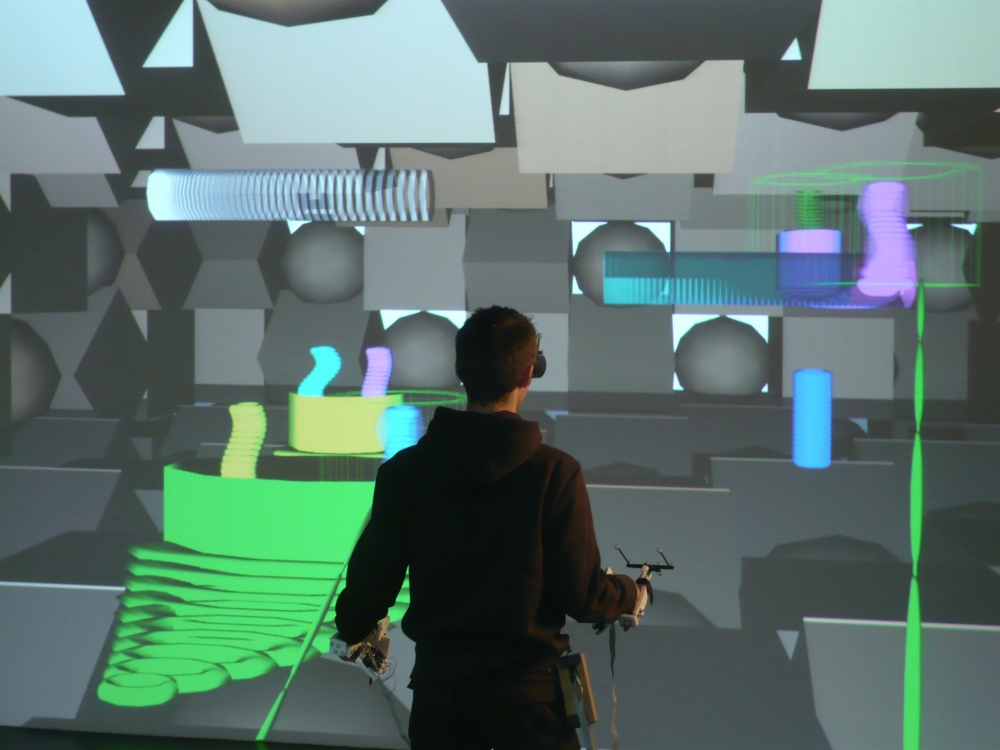
\includegraphics[scale=0.3]{image/drile.jpg}
\caption{Picture of a musician using DRILE}
\label{drile}
\end{figure}

\paragraph{}
Maintenant qu'un instrument de musique 3D a été défini, le concept d'immersion et d'interactivité doivent être définis.
\newpage
\section{Immersion}

\paragraph{}
L'immersion est un état psychologique où le sujet cesse de se rendre comtpe de son propre état physique. Le concept d'immersion est très important en réalité virtuelle. Par exemple pour la percussion aérienne cela reviendrait à l'état atteind par le musicien lorsque celui ci ne réfléchit plus consciemment à la disposition des formes avec lesquelles il interragit. Le musicien sera alors immergé dans cette scène 3D que constitue la disposition des formes de la percussion aérienne.

\paragraph{}
Ainsi pour immerger un utilisateur, il est possible de jouer sur plusieurs paramètres. Ceux ci sont très liés aux sens du corps humain. Dans le cadre de notre projet nous nous intéresserons surtout à la vision, et tout particulièrement aux dispositifs de rendu de la 3D.

\paragraph{}
L'interactivité a une part importante dans l'aspect immersif d'un système. L'utilisateur a d'autant plus le sentiment d'immersion dans un monde virtuelle si celui ci réagit instantanément à ses actions. Ceci nous amène a définir les contrôles d'un instrument de musique 3D et l'importance de l'interactivité.

\section{Control}
\paragraph{}
Pour le contrôle de l'instrument de musique 3D, il est important de voir le système de deux manières. Dans un premier temps comme un instrument de musique, qui donc doit répondre à certaine contraintes qui permet d'assurer la précision et la qualité attendu par un musicien de son instrument. Et dans un second temps comme un système interactif immersif, c'est à dire une très grande interactivité et de tirer profits un maximum des caractéristiques de l'être humain (retour visuelle immersif et retour haptique).

\paragraph{}
Pour la manipulation d'un instrument de musique, la segmentation de la gestuel faite par Cadoz \cite{cadoz1999musique} est très pertinente. Cadoz définit trois types de gestes:

\begin{itemize}
\item les gestes de sélection : action de sélection du musicien d'un composant de l'instrument plutôt qu'un autre, par exemple dans le cas d'un violon cela revient à choisir une corde plutôt qu'une autre.
\item les gestes de modification : action qui modifit l'état de l'instrument, dans le cas d'une guitare cela revient à utiliser sa main gauche pour presser une ou des cordes sur l'une des cases du manche.
\item les gestes d'excitation : action qui génère directement et physiquement le son, qui revient à pincer une corde dans le cas d'une guitare. C'est ce geste qui est soumis à l'expression de l'artiste.
\end{itemize}

\paragraph{}
Mais il ne faut pas oublier le caractère immersif du système, celui impose que l'utilisateur ait un certain confort de manipulation. L'immersion visuelle est souvent améliorer grâce à un suivi de tête à l'aide d'une Kinect. Ceci permet d'adapter la projection en fonction de la position de la tête de l'utilisateur et cela augmente l'impression d'immersion.
Des boutons de pressions à retour haptique augmentent aussi la conscience des actions de l'utilisateur, donc sa précision d'action.

\paragraph{}
Nous verrons dans la suite de ce rapport que Florent Berthaut s'est posé toutes ces questions lorsqu'il a conçu Piivert \cite{berthaut2010piivert} pour contrôler le DRILE.

\paragraph{}
Maintenant que le concept d'instrument de musique 3D est bien défini, nous allons pouvoir nous focaliser sur les techniques de rendu 3D qui nous intèressent plus particulièrement vis à vis de notre sujet.

